%\documentclass[12pt, amstex, letterpaper] {report} %{article}


\usepackage[margin=1in]{geometry}
\topmargin -0.5in \textwidth 6.5in \textheight 9in
\footskip .5in
\headheight 0.3in


\usepackage{Sweave}

\DefineVerbatimEnvironment{Sinput}{Verbatim} {xleftmargin=0em,frame=single}
\DefineVerbatimEnvironment{Soutput}{Verbatim} {xleftmargin=0em,frame=single}

\usepackage{amssymb, mathrsfs, amsmath, amsfonts}
\usepackage{enumerate, comment}
\usepackage{hyperref, natbib,apalike, float} %cite
\usepackage{color, multirow, setspace, fancyhdr,graphicx}
\usepackage{undertilde}
\usepackage[bottom]{footmisc}
\usepackage{graphicx}
\usepackage{framed}
\usepackage{subcaption}
\usepackage{amsthm}

%\doublespacing
\pagestyle{empty}
\pagestyle{fancy}
\lhead{ }
%\rhead{May 2016}
\fancyfoot{ }
\rfoot{Dissertation $|$ \thepage}
\lfoot{Chris Vanlangenberg}
\date{}

\includecomment{comment}

\newtheorem{theorem}{Theorem}[section]
\newtheorem{defn}{Definition}[section]
\newtheorem{prop}{Proposition}
\newcommand{\pro}[1]{\begin{prop}{#1}\end{prop}}

%\newtheorem{proof}{proof}
\newtheorem{rmk}{Remark}
\newcommand{\rmark}[1]{\begin{rmk}{#1}\end{rmk}}

\numberwithin{equation}{section}
\renewcommand{\footrulewidth}{0.1pt}
\renewcommand{\headrulewidth}{0.1pt}


\newcommand{\eqn}[1]{\begin{equation}{#1}\end{equation}}

\newcommand{\beq}{\begin{equation}}
\newcommand{\eeq}{\end{equation}}
%\renewcommand\refname{Literature}
\newcommand{\blue}[1]{\textcolor{blue}{\emph{#1}}}
\newcommand{\red}[1]{\textcolor{red}{\emph{#1}}}
\newcommand{\twoc}[2]{{\textcolor{blue}{#1}} and {\textcolor{red}{#2}}}


\newcommand{\xn}{x_1,\ldots, x_n}
\newcommand{\Xn}{X_1,\ldots, X_n}
\newcommand\floor[1]{\lfloor{#1}\rfloor}
\newcommand\ceil[1]{\lceil{#1}\rceil}

\newcommand{\X}{\mathcal{X}}
\newcommand{\Sp}{\mathbb{S}}
\newcommand{\R}{\mathbb{R}}
\newcommand{\C}{\mathbb{C}}
\newcommand{\pd}{positive definite }



\newcommand{\code}[1]{{\small\texttt{#1}}}
\newcommand{\pkg}[1]{{\normalfont\textsf{#1}}}
\newcommand{\var}[1] {{\normalfont\textbf{#1}}}
\newcommand{\Cm}{$C_m(\phi_P, \phi_Q)\ $}

\newcommand{\jun}{\cite{JunStein2008}}
%
%\begin{document}


%%-------------------------Random process on sphere---------------------------------------%%

%%------------------------------------------------------------------%%
\section{Random Process on a Sphere}
%%------------------------------------------------------------------%%
	
Suppose the process $\{X(P): P\in \Sp^2\}$ ($\Sp^2$ unit sphere), defined in a common probability space, where $P=(\lambda, \phi) \in \Sp^2$ with longitude $\lambda \in [-\pi, \pi)$ and latitude $\phi \in [0, \pi]$, is continuous in quadratic mean with respect to the location $P$ and has finite second moment. Then it can be represented by spherical harmonics \citep{Jones1963, LiNorth1997, Huang2012}, with the sum converging in mean squares:
	\[
	X(P) = \sum_{\nu=0}^\infty \sum_{m=-\nu}^{\nu} Z_{\nu,m} e^{i m \lambda} P_{\nu}^m (\cos \phi).
	\]
Here $P_{\nu}^m(\cdot)$ are normalized associated Legendre polynomials such that their squared integral on $[-1, 1]$
is 1, and $Z_{\nu,m}$ are complex-valued coefficients satisfying	
	\[
	Z_{\nu,m} = \int_{\Sp^2} X(P) e^{-im \lambda} P_{\nu}^m (\cos \phi) d P.
	\]
Without loss of generality, we suppose that the process $X(P)$ is with zero mean, which implies $E(Z_{\nu,m}) = 0$. Let $P = (\lambda_P, \phi_P)$ and $Q=(\lambda_Q, \phi_Q)$ be two arbitrary locations on the sphere, the covariance function of the process is given by
	\begin{eqnarray*} \label{rpq_1}
		R(P, Q) &=& \mbox{E}(X(P) \overline{X(Q)}) \\
		&=& \sum_{\nu=0}^\infty \sum_{\mu=0}^\infty \sum_{m=-\nu}^{\nu} \sum_{n=-\mu}^{\mu} \mbox{E}(Z_{\nu,m} \overline{Z}_{\mu,n}) e^{im \lambda_P} P_{\nu}^m(\cos \phi_P) e^{-i n \lambda_Q} P_{\mu}^n (\cos \phi_Q),
	\end{eqnarray*}
where $\bar{Z}$ denotes the complex conjugate of $Z$. Note that the continuity of $X(P)$ on every point $P$ implies that $R(P, Q)$ is continuous at all pairs of $(P, Q)$ \citep[page 83]{Leadbetter1967}.

	%%------------------------------------------------------------------%%
	\subsection{Homogeneous Covariance Functions on the Sphere}
	%%------------------------------------------------------------------%%
	
Under the assumption of homogeneity (or isotropy), the covariance function of a random process $X(\cdot)$ on $\Sp^2$ is invariant under rotations. More specifically, a homogeneous random process on the sphere satisfies
	\begin{eqnarray*}
	E(X(P)) &=& \mu, \quad \mbox{for any } P \in \Sp^2, \\
		Cov(X(P),X(Q)) &=& C(\theta_{PQ}),
	\end{eqnarray*}
where $\theta_{PQ}$ is the spherical angle between two locations $P, Q$, given by 
	\begin{eqnarray*}
		\theta_{PQ}  = \arccos\left(\sin(\phi_P)\sin(\phi_Q) + \cos(\phi_P)\cos(\phi_Q)\cos(\lambda_P-\lambda_Q)\right).
	\end{eqnarray*}
Parallel to the requirement for a valid covariance function in $\R^d$, a valid covariance function $C(\cdot)$ on the sphere must be non-negative definite, {\em i.e.,}
	\begin{eqnarray*}
	\sum_{i,j=1}^{N} a_i a_j C(\theta_{P_iP_j}) \ge 0,
    \end{eqnarray*}
for any integer $N$, any constants $a_1, a_2, \ldots, a_N$, and any locations $P_1, P_2, \ldots, P_N \in \Sp^2$. \\

According to \cite{schoenberg1942}, a real continuous function $C(\theta)$ is a valid homogeneous covariance function on the sphere ($\Sp^2$) if and only if it can be written in the following form:
	\begin{eqnarray*} \label{covs2_sum}
	C(\theta) = \sum_{k = 0}^\infty c_k P_k(\cos\theta), \quad \theta \in [0,\pi],
	\end{eqnarray*}
where $P_k(\cdot)$ is the Legendre polynomial, $\forall c_k\ge 0$ and $\sum_k c_k < \infty$. A general result of the above representation on $\Sp^d\ (d > 2)$ can also be found in \cite{schoenberg1942}. \\
	
Note that the Legendre polynomials $P_k(\cdot)$ are orthogonal in the following sense:
	\[
		\int_{-1}^{1} P_{n}(x)P_{m}(x)dx = \frac{2}{2n+1}\delta_{(n,m)}.
	\]
Hence the coefficients $c_k$ can be obtained as
	\beq \label{covs2_coef}
	c_{k} = \frac{2k+1}{2}\int_0^{\pi} C(\theta)P_{k}(\cos\theta)d\theta. \quad k = 0,1,2,\ldots
	\eeq
One can directly use the above integral to evaluate the validity of a homogenous covariance function on the sphere by checking if $c_k$ is non-negative for all k and $\sum_k c_k < \infty$ . \\
	
The construction of covariance models is critical for spatial prediction. However, the covariance models that are valid on $\R^d$ may not be valid on the sphere ($\Sp^2$). For example, \cite{HuangZhangRobeson2011} evaluated the validity of commonly used \cov models that are valid on $\R^d$ and summarized their findings in Table \ref{tab:cov_sphere}.

	\begin{table}[H]
		\label{valid_cov_models}
		\centering
		\caption [Validity of Covariance Functions on the Sphere]{Validity of covariance functions on the sphere, $a >0,\theta \in [0,\pi]$}
		\label{tab:cov_sphere}
		\vskip 16pt
		\begin{tabular}[htb]{lll} \hline \hline
			Model & Covariance function & Valid on $\Sp^2$           \\   \hline Spherical  &
			$\left(1-\frac{3\theta}{2a} + \frac{1}{2}
			\frac{\theta^3}{a^3}\right){\bf 1}_{(\theta \le a)}$ & Yes   \\
			[2ex]
			Stable     & $\exp\left\{-\left(\frac{\theta}{a}\right)^\alpha\right\}$ & Yes for $\alpha \in (0,1]$  \\
			      &                     & No for $\alpha \in (1,2]$ \\ [2ex] \hspace{0.2in} Exponential &
			$\exp \{-\left(\frac{\theta}{a}\right) \}$ & Yes \\ [2ex]
			\hspace{0.2in} Gaussian & $\exp\left\{-\left(\frac{\theta}{a} \right)^2
			\right\}$  & No \\ [2ex]
			Power$^*$  & $c_0 - (\theta/a)^\alpha$ & Yes for  $\alpha \in (0,1] $  \\
			& & No for $\alpha \in (1,2]$ \\ [2ex]
			Radon transform of order 2         & $e^{-\theta/a}(1+\theta/a)$ &
			No        \\ [2ex] Radon transform of order 4         &
			$e^{-\theta/a} (1+\theta/a+\theta^2/3a^2)$  & No  \\ [2ex] Cauchy &
			$(1+\theta^2/a^2)^{-1}$ &  No      \\ [2ex] Hole - effect & $\sin
			a\theta / \theta$ & No    \\ \hline \hline
		\end{tabular}
	\vskip 8pt	
$^*$When $\alpha \in (0,1]$, the power model is valid on the sphere  for some $c_0 \ge \int_0^\pi (\theta/a)^{\alpha} \sin \theta d \theta$.
		\end{table}
		 
Furthermore, \cite{Gneiting2013} showed that the Mat$\acute{e}$rn covariance function is only valid on the sphere when the smoothness parameter $\nu\in(0,1/2]$. Another way of constructing a valid homogeneous covariance function on the sphere is by using the valid covariance function in $\R^3$. Specifically, \cite{Yadrenko1983} showed that if $K(\cdot)$ is a valid isotropic covariance function on $\R^3$ then
\[
	C(\theta) = K(2\sin(\theta/2))
\]
is a valid isotropic covariance function on the unit sphere, where $\theta$ is the greatest circle distance on the sphere.
			
		%%------------------------------------------------------------------%%
		\subsection{Variogram on a Sphere}
		%%------------------------------------------------------------------%%
			
Parallel to the case of circle, if a random process $X(\cdot)$ on a sphere is intrinsically stationary on $\Sp^2$, then one has $E(X(P))=\mu$, an unknown constant for all $P\in \Sp^2$ and the variogram function between any two locations $P, Q \in \Sp^2$ depends only on the spherical angle $\theta_{PQ}$	
		\[
			Var(X(P)-X(Q)) = 2\gamma(\theta_{PQ}), \quad \forall P, Q \in \Sp^2.
		\]
		The variogram function is conditionally negative definite, that is,
		\[
			\sum_{i,j=1}^{N} a_i a_j 2\gamma(\theta_{P_iP_j}) \le 0,
		\]
for any integer $N$, any constants $a_1, a_2, \ldots, a_N$ with $\sum_i a_i = 0$, and any locations $P_1, P_2, \ldots P_N \in \Sp^2$. Immediately from \eqref{covs2_sum}, for a continuous function $2\gamma(\cdot)$ with $\gamma(0)=0$, the variogram is negative definite if and only if
		\beq
		\gamma(\theta) = \sum_{k = 0}^\infty c_k(1-P_k(\cos\theta)), \quad \theta \in [0,\pi]
		\eeq
where $P_{k}(\cdot)$ are Legendre polynomials, $\forall c_k\ge 0$ and $\sum c_k < \infty$. \\
			
It is known that in $\R^d$, one can always obtain the variogram from the stationary covariance function with $\gamma(\theta) = C(0) - C(\theta)$ but not the converse. However, in $\Sp^2$ \cite{Yaglom1961} argued that for a valid $\gamma(\theta), \theta \in [0,\pi]$ one can always construct the covariance function $C(\theta)=c_0-\gamma(\theta)$ for some $c_0 \ge \int_0^{\pi} \gamma(\theta)\sin(\theta)d\theta$. \\
			
Here is the outline of this chapter. We first introduce axially symmetric random processes on the sphere and the representation for the covariance function. Next, we propose parametric models to generalize some of existing parametric models to capture the variation across latitudes when modeling the covariance structure of axially symmetric processes on the sphere. Finally, we discuss the properties of the cross-covariance and cross-variogram estimators based on the Method of Moments.
		
\vskip 8pt		
		%%------------------------------------------------------------------%%
		\section{Axial Symmetry}
		%%------------------------------------------------------------------%%

For an axially symmetric process $X(P), P \in \Sp^2$ on the sphere, the covariance function $R(P,Q)$ at two locations $P=(\phi_P, \lambda_P), Q=(\phi_Q,\lambda_Q) \in \Sp^2$ is given by 					 
\[
R(\phi_P, \phi_Q, \lambda_P, \lambda_Q) = R(\phi_P, \phi_Q, \lambda_P-\lambda_Q).
\]
Following the discussion given by \cite{Stein2007, Huang2012}, the covariance function can be expressed as the following:					
		\begin{eqnarray} \label{axially-symmetry-cov}
			R(P,Q)  & = & R(\phi_P, \phi_Q, \lambda_P-\lambda_Q) \nonumber \\
			& = & \sum_{m=-\infty}^{\infty} \sum_{\nu=|m|}^\infty \sum_{\mu=|m|}^\infty f_{\nu,\mu,m} e^{im (\lambda_P-\lambda_Q)} P_{\nu}^m(\cos \phi_P) P_{\mu}^m (\cos \phi_Q),
		\end{eqnarray}
where the matrix $F_m(N) = \{ f_{\nu,\mu,m} \}_{\nu,\mu=|m|,|m|+1, \ldots, N }$ must be positive definite for all $N \ge |m|$ and $f_{\nu,\mu, m} = \overline{f}_{\mu, \nu, m}$ for each fixed integer $m$. Furthermore, if we denote
\[
C_m(\phi_P, \phi_Q) = \sum_{\nu=|m|}^\infty \sum_{\mu=|m|}^\infty f_{\nu,\mu,m} P_{\nu}^m(\cos \phi_P) P_{\mu}^m (\cos \phi_Q),
\]
then 				
		\beq \label{R(PQ)-01}
		R(P,Q) = R(\phi_P,\phi_Q,\Delta\lambda) = \sum_{m = -\infty}^{\infty}e^{im\Delta\lambda}C_m(\phi_P,\phi_Q), \quad m=0, \pm 1, \pm 2,...,
		\eeq
where $\Delta\lambda = \lambda_P - \lambda_Q \in [-\pi, \pi]$ and $\phi_P, \phi_Q \in [0,\pi]$. Here the complex bivariate continuous function \Cm has the following properties:

		\begin{itemize}
			\item Hermitian and positive definite.
			\item $\sum_{m = -\infty}^{\infty}|C_m(\phi_P,\phi_Q)|<\infty$ for any $\phi_P, \phi_Q \in [0, \pi]$.
		\end{itemize}
One can use the inverse Fourier transformation to derive $C_m(\phi_P, \phi_Q)$ based on $R(P,Q)$, 				
		\[
			C_m(\phi_P, \phi_Q) = \frac{1}{2\pi}\int_{-\pi}^{\pi} R(\phi_P, \phi_Q, \Delta\lambda)e^{-im\Delta\lambda} d\Delta\lambda. 
        \]
Let $C_m(\phi_P, \phi_Q) = C_m^R(\phi_P, \phi_Q) + i C_m^I(\phi_P, \phi_Q)$. From \cite{Huang2012}, if a random process is real-valued, its corresponding covariance function $R(P,Q)$ is also real-valued, and so we have \Cm $= \overline{C_{-m}(\phi_P,\phi_Q)}$. The covariance function $R(P,Q)$ on the sphere given by \eqref{R(PQ)-01} can then be simplified as the following:
			\begin{eqnarray*}
				R(P,Q) &=& C_0(\phi_P,\phi_Q) + \sum_{m=1}^{\infty} e^{-im\Delta\lambda}C_{-m}(\phi_P,\phi_Q) +  \sum_{m=1}^{\infty} e^{im\Delta\lambda}C_m(\phi_P,\phi_Q) \\
				% &=& C_0(\phi_P,\phi_Q) + \sum_{m=1}^{\infty} c_m e^{-im\Delta\lambda}( C_m^{R}(\phi_P,\phi_Q) - i C_m^{I}(\phi_P,\phi_Q)) \\
				% & &  + \sum_{m=1}^{\infty}c_m e^{im\Delta\lambda}( C_m^{R}(\phi_P,\phi_Q) + iC_m^{I}(\phi_P,\phi_Q)) \\
				&=& C_{0}^{R}(\phi_P,\phi_Q)+2 \sum_{m=1}^{\infty}[\cos(m\Delta\lambda)C_{m}^{R}(\phi_P,\phi_Q)-\sin(m\Delta\lambda)C_{m}^{I}(\phi_P,\phi_Q)].
			\end{eqnarray*}
			
			
			%%------------------------------------------------------------------%%
			\subsection{Longitudinally Reversible Processes}
			%%------------------------------------------------------------------%%
If we further assume that the covariance function $R(P, Q)$ of an axially symmetric process satisfies
			\beq
			R(\phi_P, \phi_Q, \lambda_P-\lambda_Q) = R(\phi_P, \phi_Q, \lambda_Q-\lambda_P),
			\eeq
we then call the underlying process to be longitudinally reversible (\cite{Stein2007}). Now the covariance function $R(P, Q)$ of a real-valued longitudinally reversible process reduces to			
			\[
				R(P,Q) = \sum_{m=0}^{\infty} C_m(\phi_P,\phi_Q)\cos(m\Delta\lambda).
			\]
as \Cm is real so that we have $C_{-m}(\phi_P,\phi_Q)=C_m(\phi_P,\phi_Q)$  and \Cm $= \overline{C_{-m}(\phi_P,\phi_Q)}$.

\vskip 16pt
				
%%------------------------------------------------------------------%%
\section{Proposed Parametric Models}
%%------------------------------------------------------------------%

As discussed in Section 4.2, many covariance models valid in $\R^d$ might not be valid in $\Sp^2$. Therefore, it is necessary to develop parametric models that possibly reflect the topological structure of compactness of a sphere. Although the Mat\'{e}rn covariance model has been often used to model global data in recent years, it has some drawbacks. For example, it has been shown that the homogeneous Mat\'{e}rn covariance model is not valid when the smoothness parameter is larger than 0.5. Further modifications have been proposed e.g., (\citealp{Li2013, JunStein2008, JeongJun2015}. \cite{Huang2012} discussed a new representation for the covariance structure of an axially symmetric process. Based on the parametric form of $C_m(\phi_P, \phi_Q)$, they proposed some parametric covariance models.
					
The covariance function on sphere, $R(P,Q)$,  given in \eqref{R(PQ)-01}, is clearly a function of both latitudes and the difference of longitudes. 
			% \[
			% 	R(P,Q) = f(\Delta\lambda, \phi_P,\phi_Q).
			% \]
If we assume that in \eqref{R(PQ)-01} $C_m(\phi_P, \phi_Q) = a_m \tilde{C}(\phi_P - \phi_Q)$ only depends on the difference between $\phi_P$ and $\phi_Q$, such that $C_1(\Delta\lambda) = \sum_{m=-\infty}^{+\infty}a_me^{im\Delta\lambda}$ exists, then $R(P, Q) = C_1(\Delta \lambda)\tilde{C}(\phi_P - \phi_Q)$. This is a simple separable model as given in \cite{HuangZhangRobeson2011}. Here is an example when both covariance components are exponential
			\[
				R(P, Q) = c_0e^{-a|\Delta \lambda|}e^{-b|\phi_P - \phi_Q|},
			\]
where $c_0 > 0$, and both $a>0$ and $b>0$ are defined as decay parameters in longitude and latitude, respectively. However, the separable models are not capable to capture the covariance structure of the entire sphere since it obvious also assumes the stationarity across latitudes. \cite{Huang2012} further proposed some non-separable covariance models by carefully choosing functions for $C_m(\phi_P, \phi_Q)$ that are valid on the sphere, under which some $R(P,Q)$ are given below:
			\begin{eqnarray}
				R(P,Q) &=& Ae^{-a|\phi_P-\phi_Q|} \frac{1-p^2}{1-2p \cos\Theta+p^2}, \label{model1}  \\
				R(P,Q) &=& Ae^{-a|\phi_P-\phi_Q|} \log\frac{1}{(1-2p\cos\Theta + p^2)}, \label{model2}  \\
				R(P,Q) &=& 2Ae^{-a|\phi_P-\phi_Q|}\left(\frac{\pi^4}{90}-\frac{\pi^2\Theta^2}{12}+\frac{\pi\Theta^3}{12}-\frac{\Theta^4}{48}\right),\label{model3} 
			\end{eqnarray}
where $A > 0, 0 < p < 1, u \in R$ are all constants, $\Theta = \Delta\lambda + u(\phi_P - \phi_Q) - 2k\pi$, and $k$ is chosen such that $\Theta \in [0,2\pi]$.
First notice that all of the three covariance models (\ref{model1}, \ref{model2}, \ref{model3}) depend not only on the difference in longitudes, but on the difference in latitudes as well. As an example, we consider the model (\ref{model1}) from \cite{Huang2012}. When $\phi_P = \phi_Q$, the model reduces to
			\beq
			\nonumber
			R(\phi_P, \phi_P, \Delta \lambda) = A\frac{1-p^2}{1 - 2p\cos(\Delta\lambda)+p^2},
			\eeq
indicating all covariance functions on latitudes are the same. If we further set $\Delta \lambda = 0$, the variance of the process over all locations is given by,
			\[
			Var(X(P)) = C\frac{1+p}{1 - p},
			\]
implying a constant variance across the entire sphere. This is unrealistic, since we have seen from MSU and TOMS data that the variance highly depends on latitudes. As a generalization of the above models, we propose the following proposition.
\pro{ \label{prop_nonstationary_cov}
Let $C(\cdot) = C(x-y)$ be the stationary covariance function on $\R^d$. For simplicity, we let $f(\omega) \ge 0$ be the spectral density of $C(\cdot)$. Then
				\[
					\tilde{C}(x, y) = C_2 - C(x) - C(y) + C(x-y),
				\]
				\[
				\mbox{with }	C_2 \ge \int_{-\infty}^\infty f(\omega)d\omega > 0,
				\]
				is the non-stationary covariance function on $\R^d$.
}
\begin{proof} by Bochner's theorem, if $f(\cdot) \ge 0$ is the spectral density of the covariance function $C(\cdot)$, we have
				\[
					C(x) = \int_{-\infty}^\infty e^{-ix\omega}f(\omega)d\omega.
				\]
Now for any $N$, we choose a sequence of complex numbers $a_i, i = 1, 2, \cdots, n$, and any sequence of real numbers $t_i, i = 1, 2, \cdots, n$, taking $C_2 = \int_{-\infty}^\infty f(\omega)d\omega$,
\begin{eqnarray*}
					\sum_{i=1}^n \sum_{j=1}^n a_i \overline{a}_j \tilde{C}(t_i, t_j) &=& \sum_i \sum_j a_i \overline{a}_j (C_2 - C(t_i) - C(-t_j) + C(t_i-t_j)) \\
					&=& \sum_{i=1}^n \sum_{j=1}^n a_i \overline{a}_j \int_{-\infty}^\infty(1-  e^{-it_i\omega} - e^{it_j\omega} + e^{-i(t_i-t_j)\omega})f(\omega)d\omega \\
					&=&\int_{-\infty}^\infty f(\omega)d\omega \left|\sum_{i=1}^n a_i(e^{-it_i\omega} - 1)\right|^2 \ge 0.
\end{eqnarray*}

This proves the positive definiteness of $\tilde{C}(\cdot, \cdot)$, which concludes the proof.

\end{proof}

\noi We apply the above proposition on the following two stationary covariance functions, 						
			\begin{eqnarray*}
				C(\phi) = Ce^{-a|\phi|}, \\
				C(\phi) = C\frac{1}{\sqrt{a^2+\phi^2}},
			\end{eqnarray*}
\noi where $C > 0, a > 0$. We arrive with the following two non-stationary covariance functions.  
			\begin{eqnarray}
				\label{Cm_model1}
				\tilde{C}(\phi_P, \phi_Q) &=& C_1(C_2 - e^{-a|\phi_P|} - e^{-a|\phi_Q|} + e^{-a|\phi_P - \phi_Q|}), \\
				\label{Cm_model2}
				\tilde{C}(\phi_P, \phi_Q) &=& C_1\left(C_2 - \frac{1}{\sqrt{a^2+\phi_P^2}} - \frac{1}{\sqrt{a^2+\phi_Q^2}} + \frac{1}{\sqrt{a^2+(\phi_P-\phi_Q)^2}}\right),
			\end{eqnarray}					      		
where $C_1, a > 0,$ and $C_2 \ge 1$ to ensure the positive definiteness of the above function. When $\phi_P = \phi_Q$, both functions are actually a function of $\phi_P$:		      		
			\begin{eqnarray*}
				\tilde{C}(\phi_P, \phi_P) &=& C_1(C_2 - 2e^{-a|\phi_P|} + 1), \\
				\tilde{C}(\phi_P, \phi_P) &=& C_1\left(C_2 - \frac{2}{\sqrt{a^2+\phi_P^2}} + \frac{1}{a}\right).
			\end{eqnarray*}		
Therefore, we propose the following covariance models for axially symmetric processes on the sphere, which generalize the models given by \cite[model 1, model 4, model 5]{Huang2012}:
			\begin{eqnarray}
				R(P,Q) &=& \tilde{C}(\phi_P, \phi_Q) \frac{1-p^2}{1-2p \cos\Theta+p^2}, \label{model4} \\
				R(P,Q) &=& \tilde{C}(\phi_P, \phi_Q) \log\frac{1}{(1-2p\cos\Theta* + p^2)}, \label{model5} \\
				R(P,Q) &=& \tilde{C}(\phi_P, \phi_Q) \left(\frac{\pi^4}{90}-\frac{\pi^2\Theta^2}{12}+\frac{\pi\Theta^3}{12}-\frac{\Theta^4}{48}\right), \label{model6}
			\end{eqnarray}
where $\Theta=\Delta\lambda+u(\phi_P-\phi_Q) \in [0,2\pi ] $, $C_1 > 0, C_2 > 0, a>0, u\in \R, p\in(0,1)$. \\
					
			\begin{figure}
				\centering
				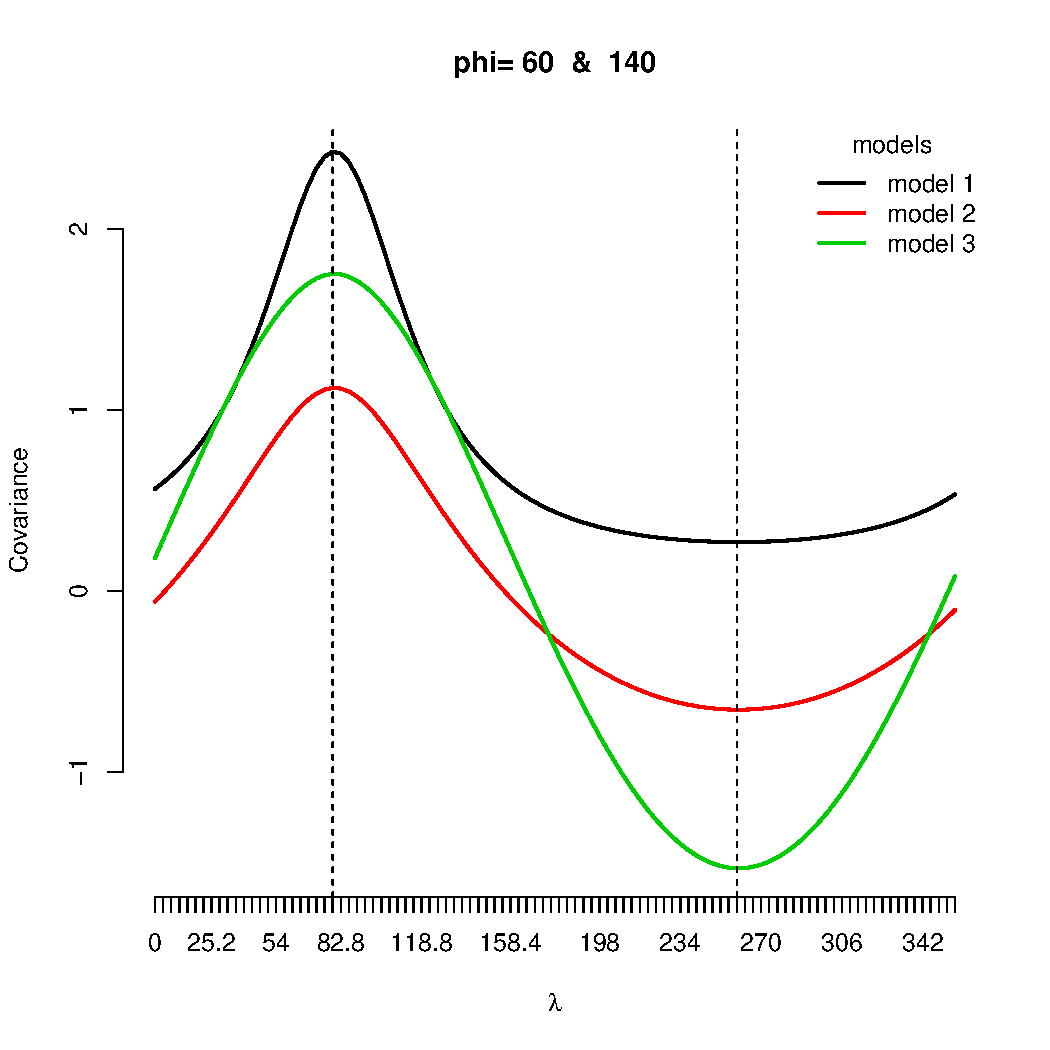
\includegraphics[width=0.7\textwidth]{graphs/all_covariance_models}
				\caption[The Covariance Between $30^0S$ and $50^0N$ (Latitudes $60^0$ and $140^0$) of Three] {The covariance between $30^0S$ and $50^0N$ (latitudes $60^0$ and $140^0$) of three covariance models with exponential family, $ i.e., \tilde{C}(\phi_P, \phi_Q)$ given by \eqref{Cm_model1} over 100 longitudes (we set $C_1 = C_2 = a = u = 1$, and $p = 0.5$).}
			\end{figure}
				
\rmark{The parameters $C_1, C_2, a, p$ are scaling parameters of the covariance functions and $u$ is a location parameter. All covariance models have a similar pattern and share one property. When there is no location shift ($u = 1$), the maximum of $R(P,Q)$ occurs at $\lambda_{max} = |\phi_P -\phi_Q|$ and the minimum of $R(P,Q)$ occurs at $\lambda_{min} = \pi + \lambda_{max}$. } 
					
			\begin{figure}
				\centering
				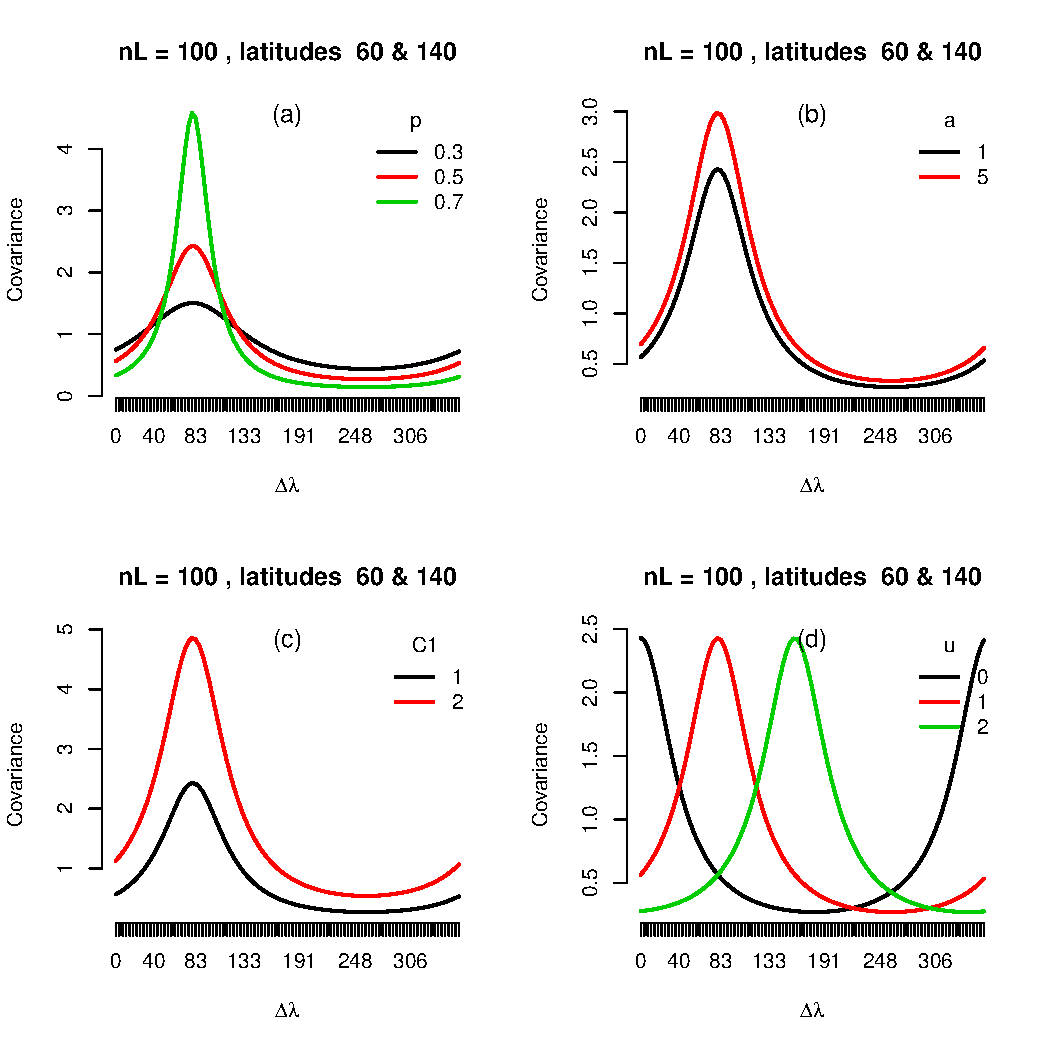
\includegraphics[width=1\textwidth]{graphs/parameters_model1_2}
				\caption[Covariance Curves for Different Parameters using Model1:] {Covariance curves for different parameters using model 1 \citep{Huang2012}:  (a)-parameter $p$, (b)-parameter $a$, (c)-parameter $C_1$ (similar pattern for parameter $C_2$), (d)-parameter $u$}
				\label{fig_parameter_comp}
			\end{figure}
			
\rmark{The scaling parameter $p$ changes rapidly at the supremum and infimum of the covariance models and parameters $C_1, C_2$, and $a$ are regular scaling parameters. The parameter $u$ is a location parameter which shifts the covariance from left to right with respect to $\Delta\lambda$) when $u>0$. When $u=0$ it provides a longitudinally reversible covariance model.}

%%------------------------------------------------------------------%%
\section{Covariance and Variogram Estimators on a Sphere}
%%------------------------------------------------------------------%%
			%In contrast the cross variogram is an even function when the process is intrinsically stationary.

The covariance function $R(P, Q)$ has also be termed as a cross covariance in the literature, as it captures the covariance of the process between points at two latitudes with longitudes separated by $\Delta \lambda \in (-\pi,\pi)$. In this section, we consider the estimator for the covariance function $R(P, Q)$ based on MOM as well as its properties. In addition, we will introduce the cross variogram function on the sphere. The unbiasedness of the cross variogram estimator based on MOM will also be discussed.


%%------------------------------------------------------------------%%
\subsection{Cross Covariance and Cross Variogram Functions}
%%------------------------------------------------------------------%%

As discussed in \cite{Wackernagel2013}, the cross covariance function, or $R(P, Q)$, can be decomposed as the following:
\begin{eqnarray*}
R(\phi_P, \phi_Q, \Delta \lambda) &=& \frac{1}{2}(R(\phi_P, \phi_Q, \Delta \lambda) + R(\phi_P, \phi_Q, -\Delta \lambda)) \\
& & + \frac{1}{2}(R(\phi_P, \phi_Q, \Delta \lambda) - R(\phi_P, \phi_Q, -\Delta \lambda)).
\end{eqnarray*}
For fixed latitudes $\phi_P$ and $\phi_Q$, the first term is an even function of $\Delta \lambda$, while the second term is an odd function of $\Delta \lambda$. We notice that, when $\phi_P \ne \phi_Q$, $R(\phi_P, \phi_Q, \Delta \lambda)$ has the following properties:
\begin{itemize}
\item $R(\phi_P, \phi_Q, \Delta \lambda) \ne R(\phi_Q, \phi_P, \Delta \lambda)$;
\item $R(\phi_P, \phi_Q, -\Delta \lambda) \ne R(\phi_P, \phi_Q, \Delta \lambda)$;
\item $R(\phi_P, \phi_Q, -\Delta \lambda) = R(\phi_Q, \phi_P, \Delta \lambda)$.
\end{itemize}
As a special case, when $\phi_P = \phi_Q$ fixed, two locations are on the same circle, the cross covariance $R(\phi_P, \phi_P, \Delta\lambda)$ is a stationary covariance function on the circle, a function depending on longitudinal difference ($\Delta\lambda$) only. \\

Now we introduce the cross variogram function on the sphere. The cross variogram function is defined as following:
\[
2\gamma(\phi_p, \phi_Q, \Delta\lambda) = E\left((X(\phi_P, \lambda+\Delta \lambda) - X(\phi_P, \lambda))(X(\phi_Q, \lambda+\Delta \lambda) - X(\phi_Q, \lambda))\right).
\]
When $\phi_P = \phi_Q$, the above expression reduces to the expression for the variogram function on the circle.\\
\noi Note that
\begin{eqnarray*}
\gamma(\phi_p, \phi_Q, \Delta\lambda) &=& \frac{1}{2}E\left((X(\phi_P, \lambda+\Delta \lambda) - X(\phi_P, \lambda))(X(\phi_Q, \lambda+\Delta \lambda) - X(\phi_Q, \lambda))\right) \\
&=& \frac{1}{2} E\left(((X(\phi_P, \lambda+\Delta \lambda) - \mu_P) - (X(\phi_P, \lambda)- \mu_P)) \right. \\
& & \left.((X(\phi_Q, \lambda+\Delta \lambda) - \mu_Q) - (X(\phi_Q, \lambda) - \mu_Q)\right) \\
&=& \frac{1}{2} \left(cov(X(\phi_P, \lambda+\Delta \lambda), X(\phi_Q, \lambda+\Delta \lambda)) \right. \\
& &- \left.cov(X(\phi_P, \lambda+\Delta \lambda), X(\phi_Q, \lambda)) \right. \\
& & \left. - cov(X(\phi_P, \lambda), X(\phi_Q, \lambda + \Delta \lambda)) + cov(X(\phi_P, \lambda), X(\phi_Q, \lambda))  \right) \\
&=& \frac{1}{2} \left(R(\phi_P, \phi_Q, 0) - R(\phi_P, \phi_Q, \Delta \lambda) - R(\phi_P, \phi_Q, -\Delta \lambda) + R(\phi_P, \phi_Q, 0)  \right) \\
&=& R(\phi_P, \phi_Q, 0) - \frac{1}{2}(R(\phi_P, \phi_Q, \Delta \lambda) + R(\phi_P, \phi_Q, -\Delta \lambda)).
\end{eqnarray*}
That is, 				
\beq
\gamma(\phi_p, \phi_Q, \Delta\lambda) =  R(\phi_p, \phi_Q, 0) - \frac{1}{2}(R(\phi_P, \phi_Q, \Delta \lambda) + R(\phi_P, \phi_Q, -\Delta \lambda)).
\eeq
We notice that the (semi-)cross variogram relates to only the even term of the cross covariance function. \cite{Wackernagel2013} argues that cross variogram might not be sufficient when there is a delayed affect, which introduces the non-zero value representing from the odd component in the cross \cov decomposition.\\

When the axially symmetric process $X(P)$ is also longitudinally reversible, that is, $R(\phi_P, \phi_Q, -\Delta \lambda) = R(\phi_P, \phi_Q, \Delta \lambda)$, we have
\begin{eqnarray*}
\gamma(\phi_p, \phi_Q, \Delta\lambda) =  R(\phi_p, \phi_Q, 0) - R(\phi_P, \phi_Q, \Delta \lambda),
\end{eqnarray*}
which is the same relationship as the one between the covariance and variogram functions on the circle.


%%------------------------------------------------------------------%%
\subsection{The MOM Cross Covariance and Cross Variogram Estimators}
%%------------------------------------------------------------------%%

We now provide the MOM estimators for the cross covariance $R(\phi_P, \phi_Q, \Delta \lambda)$ and cross semivariogram function $\gamma(\phi_P, \phi_Q, \Delta \lambda)$ of an axially symmetric process on the sphere. First for any two latitudes $\phi_P$ and $\phi_Q$ with $\{\lambda_i, i = 1, 2, \ldots, n\}$ representing the gridded longitudes on each circle (for simplicity, we assume $n = 2N$ is an even number), then the MOM estimator $\hat{R}(\phi_P, \phi_Q, \Delta \lambda)$ is given by
\beq \label{cross_covariance}
\hat{R}(\phi_P, \phi_Q, \Delta \lambda)= \frac{1}{n}\sum_{i = 1}^n (X(\phi_P, \lambda_i + \Delta \lambda) - \bar{X}_P)(X(\phi_Q, \lambda_i) - \bar{X}_Q),
\eeq
where $\Delta \lambda = 0, 2\pi/n, 4\pi/n, \cdots, 2(N-1)\pi/n$, $\bar{X}_P = \frac{1}{n}\sum_{i=1}^n X(\phi_P, \lambda_i)$, and a similar expression for $\bar{X}_Q$. 

Now we show the unbiasedness of the cross \cov estimator.	
\begin{eqnarray*}
				& & E(\hat{R}(\phi_P, \phi_Q, \Delta \lambda)) \\
				&=& \frac{1}{n}\sum_{i = 1}^n E((X(\phi_P, \Lambda_i) - \bar{X}_P)(X(\phi_Q, \lambda_i) - \bar{X}_Q)) \\
				&=& \frac{1}{n}\sum_{i=1}^n cov(X(\phi_P, \Lambda_i), X(\phi_Q, \lambda_i)) - \frac{1}{n}\sum_{i = 1}^n E((X(\phi_P, \Lambda_i) - \mu_P)(\bar{X}_Q - \mu_Q)) \\
				& & -\frac{1}{n}\sum_{i = 1}^n E((X(\phi_Q, \lambda_i) - \mu_Q)(\bar{X}_P - \mu_P)) + \frac{1}{n}\sum_{i = 1}^n E((\bar{X}_P - \mu_P)(\bar{X}_Q - \mu_Q)) \\
				&=& R(\phi_P, \phi_Q, \Delta \lambda) -E((\bar{X}_Q - \mu_Q)(\bar{X}_P - \mu_P)) - E((\bar{X}_P - \mu_P)(\bar{X}_Q - \mu_Q)) \\
				& & + E((\bar{X}_P - \mu_P)(\bar{X}_Q - \mu_Q)) \\
				&=& R(\phi_P, \phi_Q, \Delta \lambda) - cov(\bar{X}_P, \bar{X}_Q).
\end{eqnarray*}
where $\Lambda_i = \lambda_i + \Delta \lambda$ and note that,
\begin{eqnarray*}
				& & cov(\bar{X}_P, \bar{X}_Q) \\
				&=&  \frac{1}{n^2}\sum_{i = 1}^n \sum_{j=1}^n cov(X(\phi_P, \lambda_i), X(\phi_Q, \lambda_j)) \\
				&=& \frac{1}{n^2}\sum_{i = 1}^n \sum_{j=1}^n R(\phi_P, \phi_Q, (i-j)*2\pi/n) \\
				&=& \frac{1}{n^2}\sum_{i = 1}^n \sum_{j=1}^n  C_0(\phi_P, \phi_Q)  + 2\sum_{m=1}^\infty \left( C_{m, R}(\phi_P, \phi_Q) \cos(m*(i-j)*2\pi/n) \right. \\
				& & - \left. C_{m, I}(\phi_P, \phi_Q) \sin(m*(i-j)*2\pi/n) \right) \\
				&=& C_0(\phi_P, \phi_Q) + 2\sum_{m=1}^\infty C_{m, R}(\phi_P, \phi_Q) \left(\frac{1}{n^2}\sum_{i = 1}^n \sum_{j=1}^n \cos(m(i-j)*2\pi/n)\right) \\
				& & - 2\sum_{m=1}^\infty C_{m, I}(\phi_P, \phi_Q) \left(\frac{1}{n^2}\sum_{i = 1}^n \sum_{j=1}^n \sin(m(i-j)*2\pi/n)\right) \\
				&=& C_0(\phi_P, \phi_Q),
			\end{eqnarray*}			
since
			\begin{eqnarray*}
				& & \sum_{i = 1}^n \sum_{j=1}^n \cos(m*(i-j)*2\pi/n) \\
				&=& \sum_{i=1}^n \sum_{j=1}^n \left(\cos(m*i *2\pi/n)\cos(m*j*2\pi/n)\right. \\
				& & - \left.\sin(m*i *2\pi/n)\sin(m*j*2\pi/n) \right)\\
				&=& \left(\sum_{i=1}^n \cos(m*i *2\pi/n)\right)^2 - \left(\sum_{i=1}^n \sin(m*i *2\pi/n)\right)^2 = 0
			\end{eqnarray*}
and
			\begin{eqnarray*}
				& & \sum_{i = 1}^n \sum_{j=1}^n \sin(m*(i-j)*2\pi/n) \\
				&=& \sum_{i=1}^n \sum_{j=1}^n \left(\sin(m*i *2\pi/n)\cos(m*j*2\pi/n)\right. \\
				& & - \left.\cos(m*i *2\pi/n)\sin(m*j*2\pi/n) \right)\\
				&=& \left(\sum_{i=1}^n \cos(m*i *2\pi/n)\right)* \left(\sum_{i=1}^n \sin(m*i *2\pi/n)\right) \\
				& & - \left(\sum_{i=1}^n \cos(m*i *2\pi/n)\right)* \left(\sum_{i=1}^n \sin(m*i *2\pi/n)\right) = 0.
			\end{eqnarray*}
Note for any integer $m$, we have
			\[
				\sum_{k = 1}^{n} \cos(mk*2\pi/n) = \left\{\begin{array}{cc}
				0, & \mbox{for any integer $m \ne 0$,}  \\
				n, & \mbox{for $m = 0$}
				\end{array}
				\right. \mbox{ and }
				\sum_{k = 1}^{n} \sin(mk*2\pi/n) = 0.
			\]
Hence,
			\[
				cov(\bar{X}_P, \bar{X}_Q) = C_0 (\phi_P, \phi_Q).
			\]
Therefore,
			\[
				E(\hat{R}(\phi_P, \phi_Q, \Delta \lambda)) = R(\phi_P, \phi_Q, \Delta \lambda) - C_0 (\phi_P, \phi_Q).
			\]
We summarize the above calculations as the following proposition.
\begin{prop}
The MOM cross covariance estimator is biased with the constant shift given by $C_0(\phi_P, \phi_Q) = cov(\bar{X}_P, \bar{X}_Q)$. Hence, the true $R(P, Q)$ may not be identifiable based on the MOM estimator.  
\end{prop}

\vskip 8pt				
				
\rmark{When $\phi_P = \phi_Q$, the result above reduces to that for the MOM covariance estimator on the circle.}

\vskip 8pt				

\rmark{If the mean at each latitude is zero, then we can rewrite the cross covariance MOM estimator as following:			
			\[
				\hat{R}(\phi_P, \phi_Q, \Delta \lambda)= \frac{1}{n}\sum_{i = 1}^n X(\phi_P, \lambda_i + \Delta \lambda)X(\phi_Q, \lambda_i).
			\]
One can	show that this estimator is unbiased.} 

\vskip 8pt				

Next we consider the MOM cross semivariogram estimator for axially symmetric processes on the sphere.				
			\beq \label{cross_variogram}
			\hat{\gamma}(\phi_p, \phi_Q, \Delta\lambda) = \frac{1}{2n} \sum_{i=1}^n \left(X(\phi_P, \Lambda_i) - X(\phi_P, \lambda_i))(X(\phi_Q, \Lambda_i) - X(\phi_Q, \lambda_i))\right),
			\eeq
where $\Lambda_i = \lambda_i+\Delta \lambda$. We have
			\begin{eqnarray*}
				E(\hat{\gamma}_{PQ}(\Delta \lambda)) &=& \frac{1}{2n} \sum_{i=1}^n E\left(X(\phi_P, \Lambda_i) - X(\phi_P, \lambda_i))(X(\phi_Q, \Lambda_i) - X(\phi_Q, \lambda_i))\right) \\
				&=& \frac{1}{2n} \sum_{i=1}^n \left( 2\gamma(\phi_p, \phi_Q, \Delta\lambda) \right) = \gamma(\phi_p, \phi_Q, \Delta\lambda),
			\end{eqnarray*}
			which is unbiased. Here we summarize our finding as follow.

\pro{
The MOM cross semivariogram estimator is unbiased.
}

\vskip 8pt				
				
\rmark{We expect the similar result as the one in the case of ciccle for the consistency of the MOM cross semivariogram estimator on the sphere, but the proof will be more complicated. This will be one of the areas for our future research.}
				
%\end{document}			
			
